%!TEX program = xelatex
\documentclass[11pt]{beamer}

\usepackage{amsfonts}
\usepackage{amsmath}
\usepackage{blindtext}
\usepackage{enumitem}
\usepackage{hyperref}
\usepackage{colortbl}
\usepackage{fancyvrb}
\usepackage{booktabs}

\hypersetup{pdfborder = {0 0 0}}

%\usetheme{SaoPaulo}  %commented by Tao to avoid error; replace it with the line below
\usetheme{Warsaw}




\title{Welcome to CS \emph{101}!}
\subtitle{Introduction to Programming}
\author{CS101 Lecture \#1}
\date{2017-09-19}

%\setcounter{showSlideNumbers}{1} %commented by Tao to avoid error

\begin{document}
%  \setcounter{showProgressBar}{0}  %commented by Tao to avoid error
%  \setcounter{showSlideNumbers}{0}  %commented by Tao to avoid error

%Tao added below to avoid errors
\newcommand{\Enlarge}{\large}
\newcommand{\CSBase}{blue}
\newcommand{\CSGradBot}{orange}
\newcommand{\CSAltDark}{black}
\newcommand{\CSPureBase}{blue}

\newcommand{\myitem}{\item}
\newcommand{\mysubitem}{\item}


%%%%%%%%%%%%%%%%%%%%%%%%%%%%%%%%%%%%%%%%%%%%%%%%%%%%%%%%%%%%%%%%%%%%%%%%%%%%%%%%
\frame{\titlepage}

%%%%%%%%%%%%%%%%%%%%%%%%%%%%%%%%%%%%%%%%%%%%%%%%%%%%%%%%%%%%%%%%%%%%%%%%%%%%%%%%
\setcounter{framenumber}{0}
%\setcounter{showProgressBar}{1}  %commented by Tao to avoid error
%\setcounter{showSlideNumbers}{1}  %commented by Tao to avoid error

%%%%%%%%%%%%%%%%%%%%%%%%%%%%%%%%%%%%%%%%%%%%%%%%%%%%%%%%%%%%%%%%%%%%%%%%%%%%%%%%
\section{Class Structure}

%%%%%%%%%%%%%%%%%%%%%%%%%%%%%%%%%%%%%%%%%%%%%%%%%%%%%%%%%%%%%%%%%%%%%%%%%%%%%%%%
\begin{frame}[plain,c]
  \frametitle{Class Website}
  \Enlarge

  \begin{center}
    %\textcolor{CS101Base}{\Huge \texttt{go.illinois.edu/cs101}}%commented by Tao to avoid error; replace it with the line below
    \textcolor{\CSBase}{\small \texttt{\url{http://relate.intl.zju.edu.cn:8000/course/zjui-cs101-fa17/}}}

    Access to all lecture notes, homework assignments, lab materials and all other supporting materials for this class.
  \end{center}
\end{frame}

%%%%%%%%%%%%%%%%%%%%%%%%%%%%%%%%%%%%%%%%%%%%%%%%%%%%%%%%%%%%%%%%%%%%%%%%%%%%%%%%
\begin{frame}[plain,c]
  \frametitle{Class Website}
  \Enlarge

  \begin{center}
    %\textcolor{CS101Base}{\Huge \texttt{go.illinois.edu/cs101}}%commented by Tao to avoid error; replace it with the line below
    \textcolor{\CSBase}{\small \texttt{\url{http://relate.intl.zju.edu.cn:8000/course/zjui-cs101-fa17/}}}
  \end{center}
     Steps for enrolling in the course web:
     \begin{itemize}
     	\myitem Step 1. Click the ``Sign in $>>$'' button near the top of the course web.
     	\myitem Step 2. Click the button ``Sign in using your email $>>$''.   	
     	\myitem Step 3. Enter your \textbf{University email address} in the Email input box, and then click the ``Send sign-in email''.
     	\myitem Step 4. Log in to your email, click the URL included in the email titled ``Your RELATE sign-in link'' to sign in.
     	\myitem Step 5. Click the button ``View$>>$'' under course ``CS101 Fall 2017''
     	\myitem \large{Step 6. Click the ``Enroll'' button for the first time signing in, and Please fill-in your information such as name and University ID.}
     \end{itemize}
\end{frame}

%%%%%%%%%%%%%%%%%%%%%%%%%%%%%%%%%%%%%%%%%%%%%%%%%%%%%%%%%%%%%%%%%%%%%%%%%%%%%%%%
\begin{frame}
  \frametitle{Required Supplies}
  %\Enlarge %commented by Tao to avoid error

  \begin{itemize}
    %\myitem i>clicker \\ \textcolor{\CSGradBot}{\footnotesize\hspace{1em} Grades count starting Wed 08-31} \pause  %commented by Tao to avoid error
    %\myitem CodeLab account \\ \textcolor{\CSGradBot}{\footnotesize\hspace{1em} Instructions in \texttt{hw01}} \pause %commented by Tao to avoid error
    %\myitem No textbook! %commented by Tao to avoid error
    \item CodeLab account \\ \textcolor{\CSGradBot}{\footnotesize\hspace{1em} online programming platform for homeworks}
    					\\ \textcolor{\CSGradBot}{\footnotesize\hspace{1em} Instructions in \texttt{lab01} (tomorrow) for registration}
    					%\\ \textcolor{\CSGradBot}{\footnotesize\hspace{1em} Have your CodeLab account registered before the Lab session (starts on Wednesday!)}
    %\pause %commented by Tao to avoid error
     %\myitem No textbook! %commented by Tao to avoid error
  \end{itemize}
  \vspace{2mm}
  \hspace{12mm}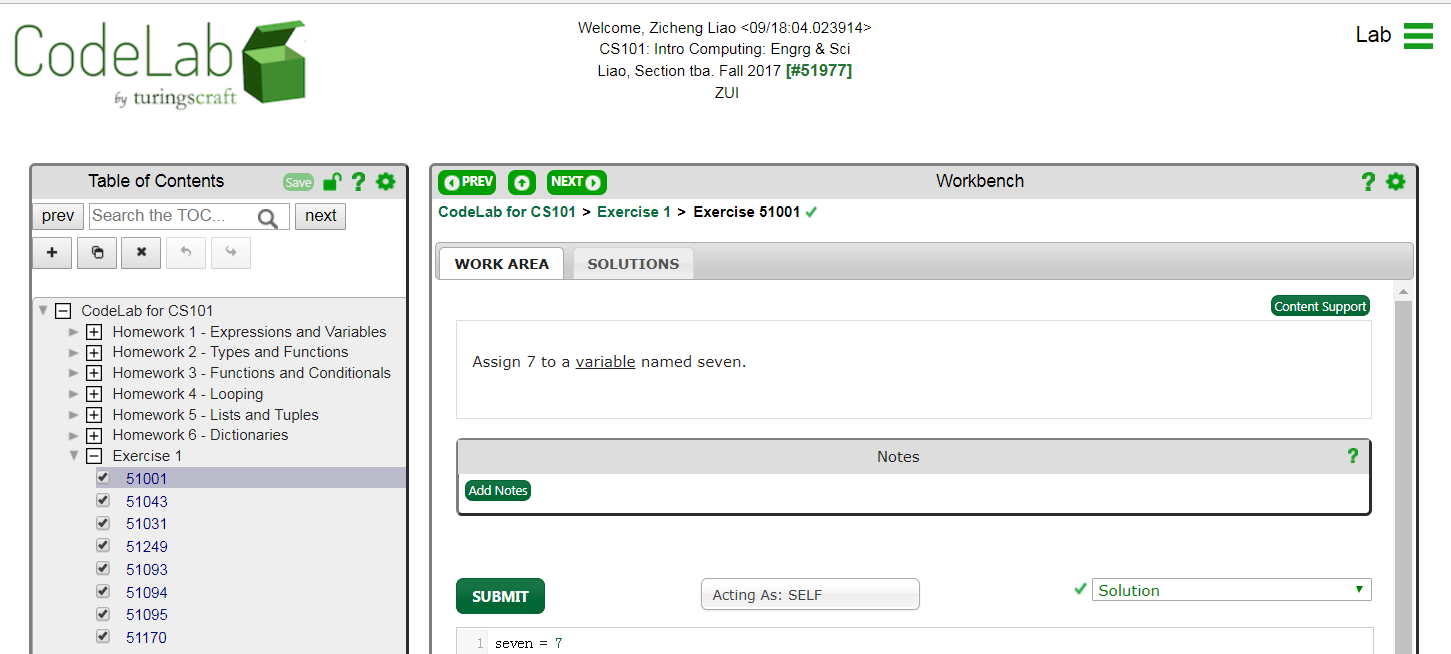
\includegraphics[height=0.4\textheight]{./img/codelab.png}
\end{frame}


%%%%%%%%%%%%%%%%%%%%%%%%%%%%%%%%%%%%%%%%%%%%%%%%%%%%%%%%%%%%%%%%%%%%%%%%%%%%%%%%
\begin{frame}
  \frametitle{Homework Policies}
  \Enlarge

  \begin{itemize}
    \myitem No late homework submissions. \pause
    \myitem All machine-generated grades are final. \pause
    \myitem Late registrants should keep up with work. \\ \textcolor{\CSGradBot}{\footnotesize\hspace{1em} Corollary:  No extensions or exceptions for late registration.} \pause
    \myitem Get help at Blackboard forum. \\ \textcolor{\CSGradBot}{\footnotesize\hspace{1em} Be civil to staff and peers.}
    							       %\\ \textcolor{\CSGradBot}{\footnotesize\hspace{1em} All posts containing solutions should be marked as private.}
  \end{itemize}
\end{frame}

\iffalse
%%%%%%%%%%%%%%%%%%%%%%%%%%%%%%%%%%%%%%%%%%%%%%%%%%%%%%%%%%%%%%%%%%%%%%%%%%%%%%%%
\begin{frame}
  \frametitle{Textbook}
  \Enlarge


  \begin{itemize}
    \myitem No required textbook
    \myitem Forget about syllabus
    %\myitem Two suggested (optional):  \\ \textcolor{\CSGradBot}{\footnotesize\hspace{1em} Hans Petter Langtangen, A Primer on Scientific Programming with Python, 5th edition. (2016).}
    %					  \\ \textcolor{\CSGradBot}{\footnotesize\hspace{1em} Stormy Attaway, MATLAB: A Practical Introduction to Programming and Problem Solving, 4th ed. (2016).} \pause

    \myitem Immense information online.
    \myitem learn to use your browser smartly
  \end{itemize}

\end{frame}
\fi

%%%%%%%%%%%%%%%%%%%%%%%%%%%%%%%%%%%%%%%%%%%%%%%%%%%%%%%%%%%%%%%%%%%%%%%%%%%%%%%%
\begin{frame}
  \frametitle{Grading}
  \begin{tabular}{*{27}{ll}}
    \toprule
    20\% & Homework \\
    25\% & Labs \\
    10\% & Lecture Participation \\
    20\% & Midterms \\
    25\% & Final Exam \\
    \bottomrule
  \end{tabular}
\end{frame}


%%%%%%%%%%%%%%%%%%%%%%%%%%%%%%%%%%%%%%%%%%%%%%%%%%%%%%%%%%%%%%%%%%%%%%%%%%%%%%%%
\begin{frame}[plain,c]
  \frametitle{Class Website}
  \Enlarge

  \begin{center}
    \textcolor{\CSBase}{\Huge Lab \#1 this Wednesday}
  \end{center}
\end{frame}





%%%%%%%%%%%%%%%%%%%%%%%%%%%%%%%%%%%%%%%%%%%%%%%%%%%%%%%%%%%%%%%%%%%%%%%%%%%%%%%%
\section{Programming}

%%%%%%%%%%%%%%%%%%%%%%%%%%%%%%%%%%%%%%%%%%%%%%%%%%%%%%%%%%%%%%%%%%%%%%%%%%%%%%%%
\begin{frame}[fragile]
  \frametitle{Early mathematics}

  \begin{tabular}{cc}
  \includegraphics[height=0.75\textheight]{./img/ybc7289.jpg}
  \includegraphics[height=0.375\textheight]{./img/ybc7289-schematic.jpg}\\
  {\tiny a Babylonian tablet from 1800-1650 BC, gives square root of 2. The best 9-decimal approx. is 1.41421356.}\\
  \textcolor{\CSBase}{\tiny \texttt{\url{http://athena.union.edu/~hemmendd/Courses/cs80/Images/}}}
  \end{tabular}
\end{frame}


\begin{frame}[fragile]
  \frametitle{Early calculation}

  \includegraphics[height=0.35\textheight]{./img/abacus.jpg} (a Roman abacus, 1st AD)\\ \pause
  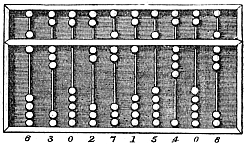
\includegraphics[height=0.35\textheight]{./img/Abacus_cn.png} \\
\end{frame}


\iffalse

%%%%%%%%%%%%%%%%%%%%%%%%%%%%%%%%%%%%%%%%%%%%%%%%%%%%%%%%%%%%%%%%%%%%%%%%%%%%%%%%
\begin{frame}[fragile]
  \frametitle{Early calculation}
  \includegraphics[height=0.25\textheight]{./img/abacus.jpg} \\
  \includegraphics[width=0.75\textwidth]{./img/pascal.jpg}
\end{frame}

%%%%%%%%%%%%%%%%%%%%%%%%%%%%%%%%%%%%%%%%%%%%%%%%%%%%%%%%%%%%%%%%%%%%%%%%%%%%%%%%
\begin{frame}[fragile]
  \frametitle{Early calculation}

  \includegraphics[height=0.75\textheight]{./img/al-khwarizmi.png}
\end{frame}

%%%%%%%%%%%%%%%%%%%%%%%%%%%%%%%%%%%%%%%%%%%%%%%%%%%%%%%%%%%%%%%%%%%%%%%%%%%%%%%%
\begin{frame}[fragile]
  \frametitle{Characteristica universalis}

  \begin{tabular}{cc}
  \includegraphics[height=0.75\textheight]{./img/wilkins.jpg}
  \includegraphics[width=0.5\textwidth]{./img/llull.png}
  \end{tabular}
\end{frame}

%%%%%%%%%%%%%%%%%%%%%%%%%%%%%%%%%%%%%%%%%%%%%%%%%%%%%%%%%%%%%%%%%%%%%%%%%%%%%%%%
\begin{frame}[fragile]
  \frametitle{Modern calculation}

  \includegraphics[height=0.75\textheight]{./img/babbage-1.jpg}
\end{frame}

%%%%%%%%%%%%%%%%%%%%%%%%%%%%%%%%%%%%%%%%%%%%%%%%%%%%%%%%%%%%%%%%%%%%%%%%%%%%%%%%
\begin{frame}[fragile]
  \frametitle{Modern calculation}

  \includegraphics[height=0.75\textheight]{./img/jacquard.jpg}
\end{frame}

%%%%%%%%%%%%%%%%%%%%%%%%%%%%%%%%%%%%%%%%%%%%%%%%%%%%%%%%%%%%%%%%%%%%%%%%%%%%%%%%
\begin{frame}[fragile]
  \frametitle{Modern calculation}

  \includegraphics[height=0.75\textheight]{./img/babbage-2.png}
\end{frame}

%%%%%%%%%%%%%%%%%%%%%%%%%%%%%%%%%%%%%%%%%%%%%%%%%%%%%%%%%%%%%%%%%%%%%%%%%%%%%%%%
\begin{frame}[fragile]
  \frametitle{Modern calculation}

  \includegraphics[height=0.75\textheight]{./img/babbage-3.jpg}
\end{frame}

%%%%%%%%%%%%%%%%%%%%%%%%%%%%%%%%%%%%%%%%%%%%%%%%%%%%%%%%%%%%%%%%%%%%%%%%%%%%%%%%
\begin{frame}[fragile]
  \frametitle{Modern calculation}

  \includegraphics[height=0.75\textheight]{./img/ibm.jpg}


\end{frame}

\fi


%%%%%%%%%%%%%%%%%%%%%%%%%%%%%%%%%%%%%%%%%%%%%%%%%%%%%%%%%%%%%%%%%%%%%%%%%%%%%%%%
\begin{frame}[fragile]
  \frametitle{Modern calculation}

  \includegraphics[height=0.6\textheight]{./img/enigma.jpg}\\
   {\small ``Enigma machine'': electro-mechanical rotor cipher machine used in World War I and World War II, invented by German engineer.}
     \textcolor{\CSBase}{\small \texttt{\url{https://en.wikipedia.org/wiki/Enigma\_machine}}}
     %\textcolor{\CSBase}{\small \texttt{\url{https://en.wikipedia.org/wiki/Cryptanalysis\_of\_the\_Enigma}}}
\end{frame}

%%%%%%%%%%%%%%%%%%%%%%%%%%%%%%%%%%%%%%%%%%%%%%%%%%%%%%%%%%%%%%%%%%%%%%%%%%%%%%%%
\begin{frame}[fragile]
  \frametitle{Modern calculation}

  \includegraphics[height=0.75\textheight]{./img/eniac.jpg}\\
  {\small ENIAC: among the earliest general-purpose electronic computers, in 1946 at University of Pennsylvania}
   \textcolor{\CSBase}{\small \texttt{\url{https://en.wikipedia.org/wiki/ENIAC}}}
\end{frame}

%%%%%%%%%%%%%%%%%%%%%%%%%%%%%%%%%%%%%%%%%%%%%%%%%%%%%%%%%%%%%%%%%%%%%%%%%%%%%%%%
\begin{frame}[fragile]
	\frametitle{Modern calculation}
	
	\includegraphics[height=0.75\textheight]{./img/illiac.jpg}\\
	{\small ILLIAC ({\bf Illi}nois {\bf A}utomatic {\bf C}omputer): 1951 - 1974. }
	\textcolor{\CSBase}{\small \texttt{\url{https://en.wikipedia.org/wiki/ILLIAC}}}
\end{frame}

\iffalse
%%%%%%%%%%%%%%%%%%%%%%%%%%%%%%%%%%%%%%%%%%%%%%%%%%%%%%%%%%%%%%%%%%%%%%%%%%%%%%%%
\begin{frame}[fragile]
  \frametitle{Instruction}

  \includegraphics[width=\textwidth]{./img/assembler-1.png}
\end{frame}

%%%%%%%%%%%%%%%%%%%%%%%%%%%%%%%%%%%%%%%%%%%%%%%%%%%%%%%%%%%%%%%%%%%%%%%%%%%%%%%%
\begin{frame}[fragile]
  \frametitle{Instruction}

  \includegraphics[width=\textwidth]{./img/assembler-2.png}
\end{frame}

%%%%%%%%%%%%%%%%%%%%%%%%%%%%%%%%%%%%%%%%%%%%%%%%%%%%%%%%%%%%%%%%%%%%%%%%%%%%%%%%
\begin{frame}[fragile]
  \frametitle{Instruction}

  \includegraphics[width=\textwidth]{./img/assembler-3.png}
\end{frame}

%%%%%%%%%%%%%%%%%%%%%%%%%%%%%%%%%%%%%%%%%%%%%%%%%%%%%%%%%%%%%%%%%%%%%%%%%%%%%%%%
\begin{frame}[fragile]
  \frametitle{Instruction}

  \includegraphics[width=\textwidth]{./img/assembler-4.png}
\end{frame}

\fi



%%%%%%%%%%%%%%%%%%%%%%%%%%%%%%%%%%%%%%%%%%%%%%%%%%%%%%%%%%%%%%%%%%%%%%%%%%%%%%%%
\begin{frame}[fragile]
  \frametitle{Instruction}

  \includegraphics[width=\textwidth]{./img/assembler-4.png}\pause
  \begin{itemize}
    \myitem an instruction consists a sequence of 8-bit signals
    \myitem byte: an 8-bit signal
    \myitem a bit: 0 or 1 (binary)
  \end{itemize}
\end{frame}


%%%%%%%%%%%%%%%%%%%%%%%%%%%%%%%%%%%%%%%%%%%%%%%%%%%%%%%%%%%%%%%%%%%%%%%%%%%%%%%%
\begin{frame}
  \frametitle{What is a program?}
  \Enlarge

  \begin{itemize} \pause
    \myitem A set of instructions a computer executes to achieve a goal.
  \end{itemize}
\end{frame}


%%%%%%%%%%%%%%%%%%%%%%%%%%%%%%%%%%%%%%%%%%%%%%%%%%%%%%%%%%%%%%%%%%%%%%%%%%%%%%%%
\begin{frame}[fragile]
  \frametitle{Programming language}

  %\begin{centering}
  \includegraphics[width=0.3\textwidth]{./img/python-logo.png} \hspace{5mm}
  
\includegraphics[width=0.3\textwidth]{./img/matlab.png}  \\
  \hspace{5mm}{\small Python}
  %\end{centering}
\end{frame}


%%%%%%%%%%%%%%%%%%%%%%%%%%%%%%%%%%%%%%%%%%%%%%%%%%%%%%%%%%%%%%%%%%%%%%%%%%%%%%%%
\begin{frame}[fragile]
  \frametitle{Programming language}
  \Enlarge
%TODO
  \begin{Verbatim}[commandchars=\\\{\}]
\textcolor{\CSAltDark}{
depth * area = volume} \pause

\textcolor{\CSPureBase}{
volume = area * depth} \pause

\textcolor{\CSAltDark}{
volume of rain / volume per raindrop}
\textcolor{\CSAltDark}{
\hspace{2cm}= number of raindrops} \pause

\textcolor{\CSPureBase}{
num_raindrops = volume_rain / volume_raindrop}
  \end{Verbatim}
\end{frame}


\iffalse
%%%%%%%%%%%%%%%%%%%%%%%%%%%%%%%%%%%%%%%%%%%%%%%%%%%%%%%%%%%%%%%%%%%%%%%%%%%%%%%%
\begin{frame}[fragile]
  \frametitle{Algorithm}
\end{frame}

%%%%%%%%%%%%%%%%%%%%%%%%%%%%%%%%%%%%%%%%%%%%%%%%%%%%%%%%%%%%%%%%%%%%%%%%%%%%%%%%
\begin{frame}[fragile]
  \frametitle{Algorithm}

  \includegraphics[height=0.75\textheight]{./img/hedge-maze.jpg}
  \\a maze?
\end{frame}

\fi

%%%%%%%%%%%%%%%%%%%%%%%%%%%%%%%%%%%%%%%%%%%%%%%%%%%%%%%%%%%%%%%%%%%%%%%%%%%%%%%%
\begin{frame}
  \frametitle{What is data?}
  \Enlarge

  \begin{itemize} \pause
    \myitem Information stored in a computer. \pause
    \myitem Encoded in binary.
  \end{itemize}
  \includegraphics[width=\textwidth]{./img/assembler-2.png}
\end{frame}

%%%%%%%%%%%%%%%%%%%%%%%%%%%%%%%%%%%%%%%%%%%%%%%%%%%%%%%%%%%%%%%%%%%%%%%%%%%%%%%%
\begin{frame}
  \frametitle{What is data?}
  \Enlarge

  \begin{itemize}
    \myitem Binary data of information of various kinds (must be interpreted):
	\begin{itemize}
	  \mysubitem values (e.g. 5) %\pause
	  \mysubitem name of a value (e.g. x = 5) %\pause
	  \mysubitem memory address (of x) %\pause
	  \mysubitem instruction (e.g. $x = y + z$) %\pause
	\end{itemize}
  \end{itemize}
  \begin{centering}
  \hspace{15mm}\includegraphics[height=0.5\textheight]{./img/dali.png}
  \end{centering}
\end{frame}

%%%%%%%%%%%%%%%%%%%%%%%%%%%%%%%%%%%%%%%%%%%%%%%%%%%%%%%%%%%%%%%%%%%%%%%%%%%%%%%%
\begin{frame}
  \frametitle{What is data?}
  \Enlarge

  \begin{itemize}
      \myitem Programs are data! \pause
      %\myitem Instructions encoded in binary.
  \end{itemize}
  \begin{center}
  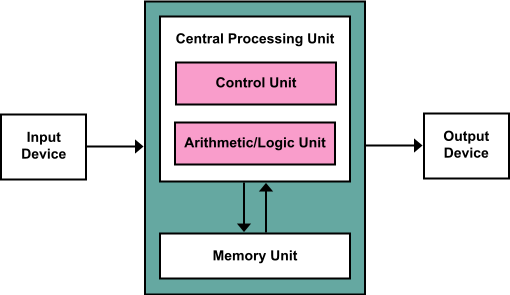
\includegraphics[width=0.6\textwidth]{./img/Von_Neumann.png}\\
  stored program machine: von Neumann architecture (1945)\\
  \textcolor{\CSGradBot}{``the concept of a machine to store in its memory a program of activities...''}
  \textcolor{\CSBase}{\small \texttt{\url{https://en.wikipedia.org/wiki/Von_Neumann_architecture}}}
  \end{center}
  %\includegraphics[width=\textwidth]{./img/assembler-4.png}
\end{frame}

%%%%%%%%%%%%%%%%%%%%%%%%%%%%%%%%%%%%%%%%%%%%%%%%%%%%%%%%%%%%%%%%%%%%%%%%%%%%%%%%
%%%%%%%%%%%%%%%%%%%%%%%%%%%%%%%%%%%%%%%%%%%%%%%%%%%%%%%%%%%%%%%%%%%%%%%%%%%%%%%%
\begin{frame}[fragile]
	\frametitle{Math calculation}
	\centering
	\includegraphics[height=0.75\textheight]{./img/2plus1.jpg}\\
	\textcolor{\CSBase}{\small \texttt{\url{http://v.baidu.com/v?word=2\%E5\%8A\%A01\%E7\%AD\%89\%E4\%BA\%8EOK+\&ct=301989888\&rn=20\&pn=0\&db=0\&s=0\&fbl=800\&ie=utf-8}}}
\end{frame}


%%%%%%%%%%%%%%%%%%%%%%%%%%%%%%%%%%%%%%%%%%%%%%%%%%%%%%%%%%%%%%%%%%%%%%%%%%%%%%%%
\begin{frame}
	\frametitle{Computational Thinking}
	\Enlarge
	
	\includegraphics[width=\textwidth]{./img/wing.jpg}
\end{frame}

%%%%%%%%%%%%%%%%%%%%%%%%%%%%%%%%%%%%%%%%%%%%%%%%%%%%%%%%%%%%%%%%%%%%%%%%%%%%%%%%

%%%%%%%%%%%%%%%%%%%%%%%%%%%%%%%%%%%%%%%%%%%%%%%%%%%%%%%%%%%%%%%%%%%%%%%%%%%%%%%%
\begin{frame}
	\frametitle{Computational Thinking}
	\Enlarge
	\begin{itemize}
		\myitem What can be done with computation? \pause
		\begin{itemize}
	  		\mysubitem paly music \pause
			\mysubitem upload photos to facebook \pause
			\mysubitem solve equations \pause
			\mysubitem predict weather \pause
            \mysubitem recognize face \pause
			\mysubitem autonomous driving
		\end{itemize}
	\end{itemize}
\end{frame}



\begin{frame}
	\frametitle{Computational Thinking}
	\Enlarge
	%\begin{itemize}
	%	\myitem What appears in everyday life is not always obvious. \pause
	%\end{itemize}
	\hspace{5mm} 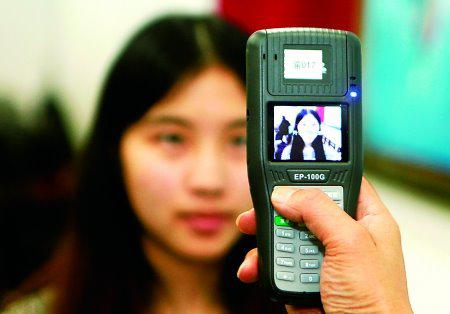
\includegraphics[width=0.7\textwidth]{./img/facepay.jpg}\\ \pause
	\begin{itemize}
	  		\mysubitem 2013, Uniqul (Finland)
			\mysubitem 2015, Alipay 8.4
	\end{itemize}
\end{frame}


\begin{frame}
	\frametitle{Computational Thinking}
	\Enlarge
	\begin{itemize}
		\myitem What can NOT be done with computation? \pause
        \begin{itemize}
    		\mysubitem sense humor (?)\pause
            \mysubitem laugh (?)
            %\mysubitem sing a song\pause
            \mysubitem ...
        \end{itemize}
		%\myitem \textcolor{\CSGradBot}{Homework: your answer to this question, and your justification (why it is so)}
	\end{itemize}
	
\end{frame}

\iffalse
%%%%%%%%%%%%%%%%%%%%%%%%%%%%%%%%%%%%%%%%%%%%%%%%%%%%%%%%%%%%%%%%%%%%%%%%%%%%%%%%
\begin{frame}[fragile]
  \frametitle{Computability Thesis}
  \centering
  \includegraphics[width=0.75\textwidth]{./img/turing-et-al.jpg}\\
  The ``Church-Turing thesis''\\
  \textcolor{\CSBase}{\tiny \texttt{\url{https://en.wikipedia.org/wiki/Church\%E2\%80\%93Turing_thesis}}}
  \begin{center}
    a hypothesis about the nature of \emph{computable} functions \\ \vspace{2mm}\pause
    %	\myitem \textcolor{\CSBase}{\tiny \texttt{\url{http://taoxie.cs.illinois.edu/sefamily.htm}}}
    \textcolor{\CSGradBot}{How about the scope of \emph{computable} functions?}
  \end{center}
\end{frame}



%%%%%%%%%%%%%%%%%%%%%%%%%%%%%%%%%%%%%%%%%%%%%%%%%%%%%%%%%%%%%%%%%%%%%%%%%%%%%%%%
\begin{frame}[fragile]
  \frametitle{Modern calculation}
 \centering
  \includegraphics[width=0.75\textwidth]{./img/turing-et-al.jpg}\\
  The ``Church-Turing thesis'' (computability thesis)

   \begin{itemize}
   	\myitem \textcolor{\CSBase}{\tiny \texttt{\url{https://en.wikipedia.org/wiki/Church\%E2\%80\%93Turing_thesis}}}
   	
   	\myitem \textcolor{\CSBase}{\tiny \texttt{\url{https://www.bigquestionsonline.com/2013/04/30/what-did-turing-establish-about-limits-computers-nature-mathematics/}}}

    	\myitem \textcolor{\CSBase}{\tiny \texttt{\url{http://www.alanturing.net/turing_archive/pages/reference\%20articles/Bio\%20of\%20Alan\%20Turing.html}}}

   %	\myitem \textcolor{\CSBase}{\tiny \texttt{\url{http://taoxie.cs.illinois.edu/sefamily.htm}}}
   \end{itemize}
\end{frame}

%%%%%%%%%%%%%%%%%%%%%%%%%%%%%%%%%%%%%%%%%%%%%%%%%%%%%%%%%%%%%%%%%%%%%%%%%%%%%%%%
\begin{frame}
	\frametitle{Computational Thinking (lol)}
	\Enlarge
	\begin{itemize}
		\myitem Four engineers traveling in a car an the car breaks down ...
		\myitem \textbf{Mechanical engineer}: ``Sounds to me as if the pistons have seized. We'll have to strip down the engine before we can get the car working again"
		\myitem \textbf{Chemical engineer}: ``it sounded to me as if the fuel might be contaminated. I think we should clear out the fuel system."
		\myitem \textbf{Electrical engineer}: ``I thought it might be an grounding problem or maybe a faulty plug lead."
		\myitem \textbf{Software/computer engineer}: ``Ummm perhaps if we all get out of the car and get back in again?"
	\end{itemize}
\end{frame}
\fi

%%%%%%%%%%%%%%%%%%%%%%%%%%%%%%%%%%%%%%%%%%%%%%%%%%%%%%%%%%%%%%%%%%%%%%%%%%%%%%%%
\begin{frame}
	\frametitle{}
	\Enlarge
	\vspace{5mm}
	Good leaders ask how to do things; great leaders ask what to do.
	
	\vspace{2mm}
	\hfill 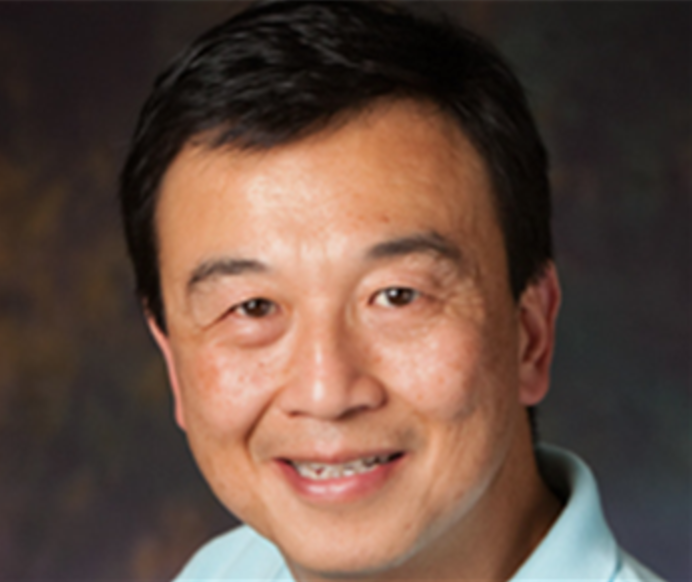
\includegraphics[width=0.3\textwidth]{./img/wenmei.png} \hspace{10mm} \\
	\small \hfill Wen-Mei Hwu/UIUC\\
\end{frame}

\iffalse
%%%%%%%%%%%%%%%%%%%%%%%%%%%%%%%%%%%%%%%%%%%%%%%%%%%%%%%%%%%%%%%%%%%%%%%%%%%%%%%%
\begin{frame}
	\frametitle{Reality in Industry: Engineering  Thinking}
	\Enlarge
	\begin{itemize}
		\myitem Researchers working on a robot arm for assembling pens.
		\myitem They face challenges, e.g., lacking sufficient accuracy.
		\myitem Any directions for solving the problem?
	
	\end{itemize}
	 \includegraphics[width=\textwidth]{./img/robotarm.jpg}
\end{frame}
\fi

%%%%%%%%%%%%%%%%%%%%%%%%%%%%%%%%%%%%%%%%%%%%%%%%%%%%%%%%%%%%%%%%%%%%%%%%%%%%%%%%

\section{Reminders}

%%%%%%%%%%%%%%%%%%%%%%%%%%%%%%%%%%%%%%%%%%%%%%%%%%%%%%%%%%%%%%%%%%%%%%%%%%%%%%%%
\begin{frame}[plain,c]
  \frametitle{Reminders}
  \Enlarge

  \begin{center}
    {\Huge Lab \#1 this Wednesday}\\ \vspace{2mm}
    \textcolor{\CSBase}{({\bf Bring your Laptop to the Lab session})}
  \end{center}
\end{frame}

\end{document}
